\newpage
\section{马尔可夫决策过程}

马尔可夫决策过程 (Markov decision process,MDP). 

\subsection{马尔可夫过程}


\begin{definition}[随机过程]
    在随机过程中, 随机现象在某时刻 $t$ 的取值是一个向量随机变量 $S_t \in \SC$, $\SC$ 为状态集合. $S_t$ 通常取决于 $t$ 之前的状态, 历史信息为 $(S_1, \dots, S_t)$, 则下一刻状态为 $S_{t+1}$ 的概率为 $P(S_{t+1}| S_1,\dots, S_t)$.
\end{definition}
随机过程 (stochastic process) 是概率论"动力学"部分. 

\begin{definition}[马尔可夫性质]
    一个随机过程被称为有马尔可夫性质 (Markov property), 当且仅当某时刻状态仅取决于上时刻的状态. i.e. 
    \begin{align*}
        P(S_{t+1}|S_t) = P(S_{t+1}| S_1,\dots, S_t)
    \end{align*}
\end{definition}

\begin{definition}[马尔可夫过程]
    马尔可夫过程 (Markov process) 指有马尔可夫性质的随机过程, 也称为马尔可夫链 (Markov chain). 用 $\braket{\SC, \PC}$ 描述一个马尔可夫过程. $\SC$ 为有限数量状态集合, $\PC$ 为状态转移矩阵 (state transition matrix). 假设有 $n$ 个状态, $\SC\in\{ s_1, s_2, \dots ,s_n \}$, 
    \begin{align*}
        \PC=\begin{bmatrix}
            P(s_1|s_1) & \cdots & P(s_n|s_1)\\
            \vdots & \ddots  & \vdots  \\
            P(s_1|s_n) & \cdots & P(s_n|s_n)
        \end{bmatrix}
    \end{align*}
    $P(s_j|s_i)=P(S_{t+1}=s_j|S_t=s_i)$ 表示从 $s_i$ 转移到 $s_j$ 的概率. 称 $P(s'|s)$ 为状态转移函数. $\PC$ 每一行和为 1. 
\end{definition}

\begin{figure}[!htb]
    \centering
    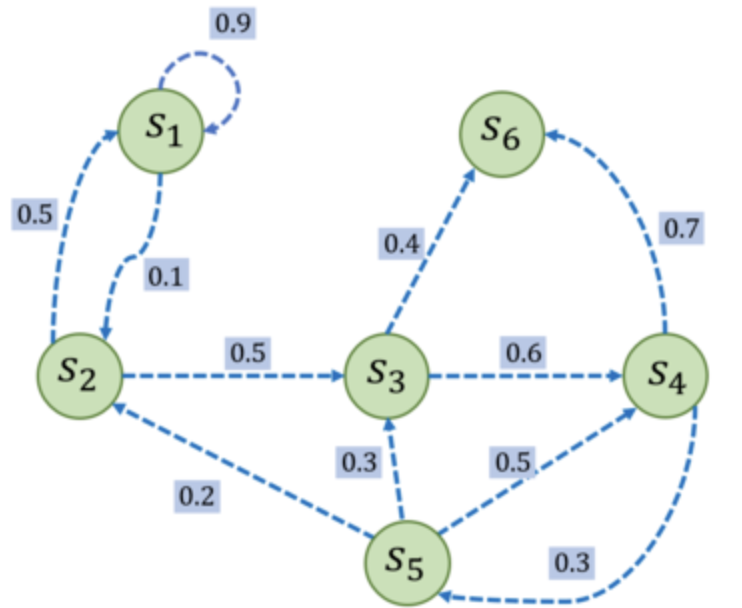
\includegraphics[width=0.618\linewidth]{pic/RL3/马尔可夫过程的一个简单例子.png}
    \caption{ \label{fig:rl3-markov} 马尔可夫过程的一个简单例子}
\end{figure}

在 \textbf{Figure} \ref{fig:rl3-markov} 中, $s_6$ 通过称为终止状态 (terminal state). 从某个状态出发, 根据状态转移矩阵生成一个状态序列 (episode), 此步称为采样 (sampling). 

\subsection{马尔可夫奖励过程}
在马尔可夫过程上加入奖励函数 $r$ 和折扣因子 (discount factor) $\gamma$, 就可以得到马尔可夫奖励过程 (Markov reward process).

\begin{definition}[马尔可夫奖励过程]
    对于一个马尔可夫奖励过程 $\braket{\SC, \PC, r, \gamma}$:
    \begin{itemize}
        \item $\SC$ 为有限状态集合.
        \item $\PC$ 为状态转移矩阵.
        \item $r$ 为奖励函数, 状态 $s$ 的奖励 $r(s)$ 指转移到该状态时可以获得奖励的期望. 
        \item $\gamma\in[0,1)$ 为折扣因子, 接近 1 的 $\gamma$ 考虑长期累积奖励, 接近 0 的 $\gamma$ 考虑短期奖励. 
    \end{itemize}
\end{definition}
引入 $\gamma$ 的原因是长期收益有不确定性, 所以希望能更快获得一些奖励. 

\begin{definition}[回报]
    在一个马尔可夫奖励过程中, 从 $t$ 刻 $S_t$ 开始, 直到终止, 所有奖励衰减之和称为回报 (return) $G_t$, 
    \begin{align*}
        G_t=R_t + \gamma R_{t+1} + \gamma^2R_{t+2} + \dots = \sum_{k=0}^\infty \gamma^k R_{t+k}
    \end{align*}
    其中 $R_t$ 表示 $t$ 课获得的奖励. 
\end{definition}

\begin{definition}[价值函数]
    在马尔可夫奖励过程中, 一个状态的期望回报, 即从这个状态出发的未来积累奖励期望, 被称为这个状态的价值 (value). 所以状态的价值组成价值函数 (value function), 
    \begin{align*}
        V(s) = \E [G_t | S_t = s]
    \end{align*}
\end{definition}

可以将价值函数展开:
\begin{align*}
    V(s) &= \E [G_t | S_t = s]\\
    &= \E [R_t + \gamma(R_{t+1} + \gamma R_{t+2} + \dots) | S_t = s] \\
    &= \E [R_t + \gamma G_{t+1} | S_t = s] \\
    &= \E [R_t | S_t = s]  + \gamma \E [ V(S_{t+1}) | S_t = s]\\ 
    &= r(s) + \gamma \sum_{s'\in S} P(s' |s) V(s')
\end{align*}
最后的结果就是贝尔曼方程 (Bellman equation), 对每个状态都成立. 若一个马尔可夫奖励过程有 $n$ 个状态, $\SC = \{ s_1, s_2, \dots, s_n \}$, 价值函数 $\VC = [V(s_1), V(s_2) ,\dots, V(s_n)]^\top$, 奖励函数 $\RC = [r(s_1) , r(s_2) , \dots , r(s_n)]^\top $, 于是有矩阵形式的贝尔曼方程
\begin{align*}
    \VC &= \RC + \gamma \PC \VC\\
    \begin{bmatrix}
        V(s_1)\\ V(s_2) \\ \vdots\\ V(s_n)
    \end{bmatrix} &= \begin{bmatrix}
        r(s_1) \\ r(s_2) \\ \vdots \\ r(s_n)
    \end{bmatrix} + \gamma \begin{bmatrix}
        P(s_1|s_1) & \dots & P(s_n|s_1)\\
        P(s_1|s_2) & \dots & P(s_n|s_2)\\
        \vdots & \ddots & \vdots \\
        P(s_1|s_n) & \dots & P(s_n|s_n)\\
    \end{bmatrix}\begin{bmatrix}
        V(s_1)\\ V(s_2) \\ \vdots\\ V(s_n)
    \end{bmatrix} 
\end{align*}

可以求 $\VC$ 解析解,
\begin{align*}
    \VC &= \RC + \gamma \PC \VC\\
    \VC &= (I-\gamma \PC)^{-1} \RC
\end{align*}
时间复杂度为 $O(n^3)$. 

\subsection{马尔可夫决策过程}

在马尔可夫奖励过程加上动作, 得到马尔可夫决策过程 (Markov decision process, MDP). 

\begin{definition}[马尔可夫决策过程]
    对于一个马尔可夫决策过程 $\braket{\SC, \AC, \PC, r,\gamma}$,
    \begin{itemize}
        \item $\SC$ 为状态集合.
        \item $\AC$ 是动作集合.
        \item $\gamma\in[0,1)$ 为折扣因子.
        \item $r(s,a)$ 为奖励函数, 同时取决于状态 $s$ 和动作 $a$. 
        \item $P(s'|s,a)$ 为状态转移函数, 表示在状态 $s$ 执行动作 $a$ 后达到状态 $s'$ 的概率. 
    \end{itemize}
\end{definition}

由船在水中漂流为例, 马尔可夫奖励过程是船在水中自由漂, 马尔可夫决策过程是有人控制船漂的方向. 

更具体的, 智能体 (agent) 根据当前状态 $S_t$ 选择动作 $A_t$, 对于状态 $S_t$ 与 动作 $A_t$, MDP 根据奖励函数和状态函数得到 $S_{t+1}$ 和 $R_t$ 并反馈给智能体. 智能体目标就是最大化累积奖励. 智能体根据状态选择动作的函数称为策略. 

\begin{definition}[策略]
    智能体的策略 (Policy) $\pi$ 表示其在状态 $s$ 下采取动作 $a\in\AC$ 的概率,
    \begin{align*}
        \pi(a|s) = P(A_t = a | S_t = s)
    \end{align*}
\end{definition}

当一个策略是确定性策略时, 其每个状态只输出一个动作; 当一个策略是随机性策略时, 每个状态的输出的动作的概率分布, 根据分布采样得到动作. 

\begin{definition}[状态价值函数]
    状态价值函数 (state-value function) $V^\pi(s)$ 表示在 MDP 中, 从状态 $s$ 出发, 遵循策略 $\pi$ 能得到的期望回报:
    \begin{align*}
        V^\pi(s) = \E_\pi [G_t | S_t= s]
    \end{align*}
\end{definition}

\begin{definition}[动作价值函数]
    动作价值函数 (action-value function) $Q^\pi(s,a)$ 表示在 MDP 中遵循策略 $\pi$ 时, 对当前状态 $s$ 执行动作 $a$ 得到的期望回报:
    \begin{align*}
        Q^\pi(s,a)&=\E_\pi [G_t | S_t =s, A_t = a]
    \end{align*}
\end{definition}

在使用策略 $\pi$ 时, 状态价值函数和动作价值函数有如下关系:
\begin{align*}
    V^\pi(s) &= \sum_{a\in\AC} \pi(a|s) Q^\pi(s,a)\\
    Q^\pi(s,a) &= r(s,a) + \gamma \sum_{s'\in\SC}P(s'|s,a)V^\pi(s')
\end{align*}

接下来推导两个价值函数的贝尔曼期望方程(Bellman Expectation Equation):
\begin{align*}
    V^\pi(s) &= \E_\pi [R_t | S_t = s]  + \gamma \E_\pi [ V^\pi(S_{t+1}) | S_t = s]\\ 
    &= \sum_{a\in\AC}\pi(a|s) \left[ r(s,a) + \gamma \sum_{s'\in\SC} p(s'|s, a)V^\pi(s') \right]\\
    Q^\pi(s,a) &= \E_\pi [R_t +\gamma Q^\pi(S_{t+1}, A_{t+1}) | S_t = s, A_t=a]\\ 
    &=r(s,a) + \gamma \sum_{s'\in\SC} p(s'|s,a)\sum_{a'\in\AC}\pi(a'|s')Q^\pi(s', a')
\end{align*}

\begin{figure}[!htb]
    \centering
    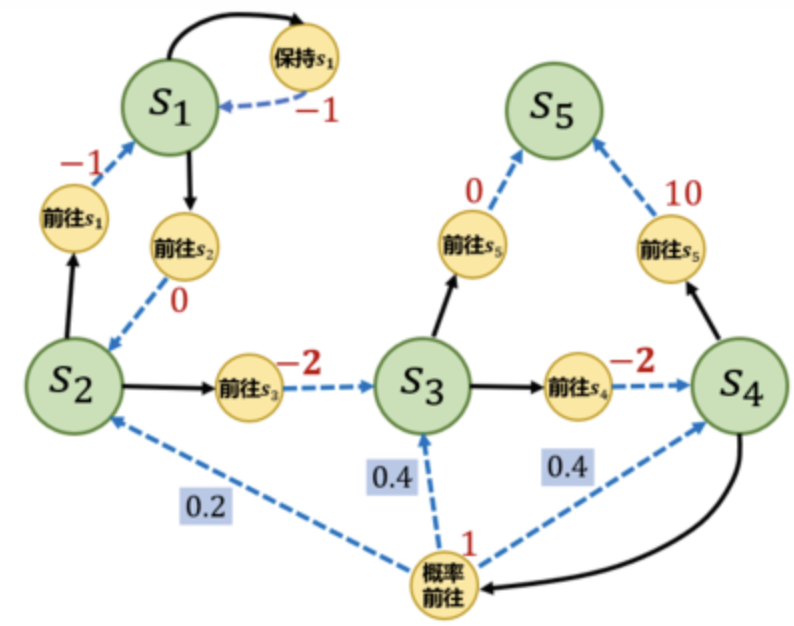
\includegraphics[width=0.618\linewidth]{pic/RL3/马尔可夫决策过程的一个简单例子.png}
    \caption{马尔可夫决策过程的一个简单例子}
\end{figure}


计算策略 $\pi$ 的状态价值函数. 我们将 MDP 转化为 MRP, 用 MRP 的方法求解状态价值函数. 
\begin{theorem}
    给定一个 MDP 和一个策略 $\pi$, 我们可以将其转化为一个 MRP.
\end{theorem}

\begin{proof}
    对于一个 MDP $\braket{\SC, \AC, \PC, r,\gamma}$,

    将策略的动作选择进行边缘化 (marginalization), 对于某个状态 $s$, 根据策略所有动作概率进行加权, 得到的奖励和可以认为是一个 MRP 在该状态下的奖励:
    \begin{align*}
        r'(s) = \sum_{a\in\AC}\pi(a|s)r(s,a)
    \end{align*}

    同理, 可以计算 MRP 的状态转移概率:
    \begin{align*}
        P'(s'|s) = \sum_{a\in\AC}\pi(a|s)P(s'|s,a)
    \end{align*}

    最后得到一个 MRP $\braket{\SC, \PC', r',\gamma}$
\end{proof}

有了状态价值函数, 就可以通过公式计算动作价值函数. 

\subsection{蒙特卡洛方法}
通过多次采样估计一个策略在一个马尔可夫决策过程中的状态价值函数. 然后再计算动作价值函数.


\subsection{占用度量}
不同策略的价值函数是不一样的, 因为即使是同一个 MDP, 不同策略访问到的状态的概率分布是不同的. 

\begin{definition}[状态访问分布]
    令一个 MDP 的初始状态分布为 $\nu_0(s)$, 用 $P_t^\pi(s)$ 表示在策略 $\pi$ 中, 智能体在 $t$ 时刻状态为 $s$ 的概率, 有 $P_0^\pi(s)=\nu_0(s)$, 以及一个策略的状态访问分布 (state visitation distribution):
    \begin{align*}
        \nu^\pi(s) = (1-\gamma)\sum_{t=0}^\infty \gamma^t P_t^\pi(s)
    \end{align*}
    $1-\gamma$ 是使概率和为 1 的归一化因子. 
    
    状态访问分布表示一个策略和 MDP 交互会访问到的状态的分布.
\end{definition}

$1-\gamma$ 为什么是归一化因子, 是因为: 
\begin{align*}
    \sum_{t=0}^\infty \gamma^t = \frac{1}{1-\gamma}
\end{align*}

状态访问分布有如下性质:
\begin{align*}
    \nu^\pi(s')=(1-\gamma)\nu_0(s') + \gamma \int P(s'|s, a)\pi(a|s)\nu^\pi(s) \,dsda 
\end{align*}

\begin{definition}[占用度量]
    一个策略的占用度量 (occupancy measure):
    \begin{align*}
        \rho^\pi(s,a) = (1-\gamma) \sum_{t=0}^\infty \gamma^t P_t^\pi(s)\pi(a|s)
    \end{align*}
    表示动作状态对 $(s,a)$ 被访问到的概率. 
\end{definition}

占用度量与状态访问分布有如下关系:
\begin{align*}
    \rho^\pi(s,a)=\nu^\pi(s)\pi(a|s)
\end{align*}

由此得出定理:
\begin{theorem}
    智能体分别以策略 $\pi_1, \pi_2$ 和同一个 MDP 交互得到占用度量 $\rho^{\pi_1}, \rho^{\pi_2}$, 有
    \begin{align*}
        \rho^{\pi_1} = \rho^{\pi_2} \iff \pi_1 = \pi_2
    \end{align*}
\end{theorem}

\begin{theorem}
    给定一合法占用度量 $\rho$, 可生成该占用度量的唯一策略为;
    \begin{align*}
        \pi_\rho(a|s) = \frac{\rho(s,a)}{\sum_{a'}\rho(s,a')}
    \end{align*}
    
\end{theorem}

\begin{proof}
    根据占用度量与状态访问分布的关系: 
    \begin{align*}
        \rho^\pi(s,a)&=\nu^\pi(s)\pi(a|s)\\
        \sum_{a'}\rho(s,a') &= \nu^\pi(s)\sum_{a'}\pi(a'|s) \\
        &= \nu^\pi(s) \\
        \therefore\ \pi(a|s)  &=\frac{\rho(s,a)}{\nu^\pi(s)} \\
        &=\frac{\rho(s,a)}{\sum_{a'}\rho(s,a')}
    \end{align*}
\end{proof}

需要合法约束是因为并非任意 $\rho$ 都能对应一个可行的策略. 具体来说:
\begin{definition}[合法占用度量]
    一个合法占用度量 $\rho$ 需要满足:
    \begin{itemize}
        \item 非负: $\forall (s,a),\ \rho(s,a)\ge 0$
        \item 流量守恒: $\forall s'\in\SC,\ s'\ne s_0$(任意非初始状态),
        \begin{align*}
            \sum_{a'}\rho(s',a')=\sum_{s,a}\rho(s,a)P(s'|s,a)
        \end{align*}
        即流入状态 $s'$ 的概率质量等于从其他状态流出到 $s'$ 的概率质量. 
        \item 初始状态约束: 对于 $\nu_0$, 有:
        \begin{align*}
            \sum_a\rho(s_0,a)=\nu_0(s_0)+\sum_{s,a}\rho(s,a)P(s_0|s,a)
        \end{align*}
        即初始状态占用度量需要考虑初始状态分布以及从其他状态转移而来的概率. 
        \item 归一化, 占用度量总和为一. 对于有限时间步, 归一化常数可能不是 $1-\gamma$.
    \end{itemize}
\end{definition}

\subsection{最优策略}
强化学习的目标通常是找到一个策略, 使智能体从初始状态出发能获得最多的期望回报. 

\begin{definition}
    当且仅当 $\forall s,\ V^\pi(s)\ge V^{\pi'}(s)$, 有 $\pi > \pi'$
\end{definition}

\begin{theorem}
    在有限状态和动作集合的 MDP 中, 至少存在一个策略不差于其他所有策略, 称这个策略为最优策略 (optimal policy), 记为 $\pi^*(s)$.
\end{theorem}

最优策略可能有多个. 

\begin{definition}[最优状态价值函数]
    最优策略都有相同的状态价值函数, 称之为最优状态价值函数:
    \begin{align*}
        V^*(s)=\max_\pi V^\pi(s),\ \forall s\in\SC
    \end{align*}
\end{definition}

\begin{definition}[最优动作价值函数]
    同理, 最优策略都有相同的动作价值函数, 称之为最优最优动作价值函数:
    \begin{align*}
        Q^*(s,a)=\max_\pi Q^\pi(s,a),\ \forall s\in \SC,a\in\AC
    \end{align*}
\end{definition}

最优状态价值函数与最优动作价值函数的关系:
\begin{align*}
    Q^*(s,a) &= r(s,a)+\gamma\sum_{s'\in\SC} P(s'|s,a)V^*(s')\\
    V^*(s)&=\max_{a\in \AC}Q^*(s,a)
\end{align*}

由此可以得到贝尔曼最优方程 (Bellman optimal equation):
\begin{align*}
    V^*(s)&=\max_{a\in\AC}\left\{ r(s,a) + \gamma \sum_{s'\in\SC} P(s'|s,a) V^*(s') \right\}\\
    Q^*(s,a) &= r(s,a) + \gamma \sum_{s'\in\SC} P(s'|s,a)\max_{a'\in\AC}Q^*(s', a')
\end{align*}